\documentclass{article}
\usepackage[margin=1in]{geometry}
\usepackage{graphicx}
\usepackage{xcolor}
\usepackage{float}
\usepackage{amsmath}
\usepackage{cite}
\usepackage{hyperref}
\graphicspath{{..} {./images}}

\definecolor{navy-blue}{rgb}{0.22,0.38,0.71}

\renewcommand{\contentsname}{\vspace*{-2\baselineskip}}

\hypersetup{
	colorlinks,
	linkcolor=black,
	urlcolor=black,
	citecolor=black
}
  		
\begin{document}
\begin{titlepage}
	\centering
	{\huge Lab 2 - Introduction to Software-Defined Radio}\\[0.25 in]
	
\includegraphics[width=0.6\textwidth]{ua_logo.png}\\[0.25 in]
	{\large \textbf{ECE 531 - Software Defined Radio\\[0.25 in]
	February 26, 2025\\[0.25 in]}}
	{\large Owen Sowatzke, osowatzke@arizona.edu\\[0.05 in]
	Department of Electrical \& Computer Engineering\\[0.05 in]
	University of Arizona, Tucson, AZ 85721\\[0.5 in]}
	\hypersetup{linkcolor=navy-blue}
	\noindent\hrulefill
	\tableofcontents
	\noindent\hrulefill
\end{titlepage}

\setlength{\parindent}{0pt}

\section{Introduction}
%Introduction to the laboratory experiment, including a brief description of the objectives and goals.

\section{Procedure}
% Detailed explanation of the laboratory experiment, including the design, implementation, and testing of the system.

\subsection{Industrial Input/Output (IIO)}
\label{section::industrial_input_output}

We can use the \texttt{iio\_info -s} command to identify the PlutoSDR device's Universal Resource Identifier (URI). We execute the provided command in an SSH terminal session connected to the embedded PlutoSDR operating system and in a local PC terminal. After executing the command in both terminals, we compare the resulting URIs.

Next, we use the \texttt{iio\_attr} command in the SSH terminal to locate the \textit{ad9361-phy} device. Once we find the device, we use the following command to verify the device name:

\begin{center}
\texttt{cat /sys/bus/iio/devices/$<$iio\_device$>$/name}
\end{center}

where \texttt{$<$iio\_device$>$} is the IIO device we find with the \texttt{iio\_attr} command. Then, we use the \texttt{iio\_attr} command to list the attributes of the \textit{ad9361-phy} device.

\subsection{MATLAB Loopback}

In this experiment, we perform a loopback test by connecting the Pluto SDR's transmit and receive ports together with a coaxial SMA cable. Once the cable is properly connected, we execute the provided \texttt{loopback.m} script to perform a physical collect. After validating that our loopback collect works, we evaluate the impact of the \textit{GainSource} (AGC) settings by testing each possible configuration: \textit{Manual}, \textit{AGC Slow Attack}, and \textit{AGC Fast Attack}. To characterize the impact of these settings, we modify the transmitted signal. We perform one collect while varying the amplitude of the signal and another collect with zero portions added to the signal. Finally, we determine what gain values are necessary to turn the receive sinusoid into a square wave (saturate the signal).

\subsection{GNU Radio Loopback}
\label{section::gnu_radio_loopback}

We can perform a similar loopback experiment using GNU Radio instead of MATLAB. For this test, we use the provided \texttt{PlutoTestSine.grc} flowchart. The lab also mentions a QT GUI Time Sink, which is not included in the provided flowchart. To meet the requirements of this experiment, we have added the time sink to the flowchart. The resulting flowchart is shown in Figure \ref{fig::gnu_radio_loopback_flowchart0}.

\begin{figure}[H]
	\centerline{\fbox{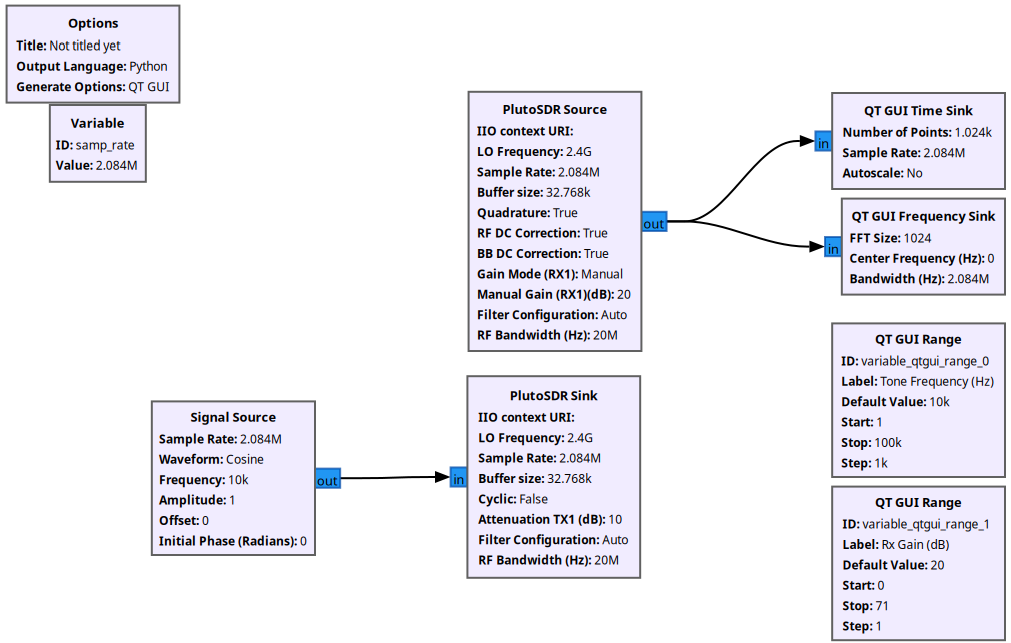
\includegraphics[width=0.6\textwidth]{gnu_radio_loopback_flowchart0.png}}}
	\caption{GNU Radio Flowchart for Loopback Test}
	\label{fig::gnu_radio_loopback_flowchart0}
\end{figure}

Before we run the flowchart, we review the properties of the PlutoSDR blocks. We specifically review the RF bandwidth and its impact on performance. Then, we describe what the "Cyclic" option does in the PlutoSDR sink. Finally, we discuss the effects of Manual Gain control in the Pluto SDR and review alternative gain control strategies.

After reviewing the PlutoSDR blocks, we run the flowchart and determine the RX gain where the signal distorts (or clips). Next, we replace the "QT Time Sink" and "QT Frequency Sink" blocks with a "QT GUI Sink" block. Using the updated block, we examine the impacts of increasing the number of averages and changing the window function. Then, we determine the transmitted RF frequency and explain how our transmitter configuration produced this frequency.

\subsection{GNU Radio as a libIIO Client}

For this experiment, we replace the PlutoSDR source and sink blocks with generic IIO blocks. The generic IIO blocks and their default values are given in Figure \ref{fig::generic_iio_blocks}.

\begin{figure}[H]
	\centerline{\fbox{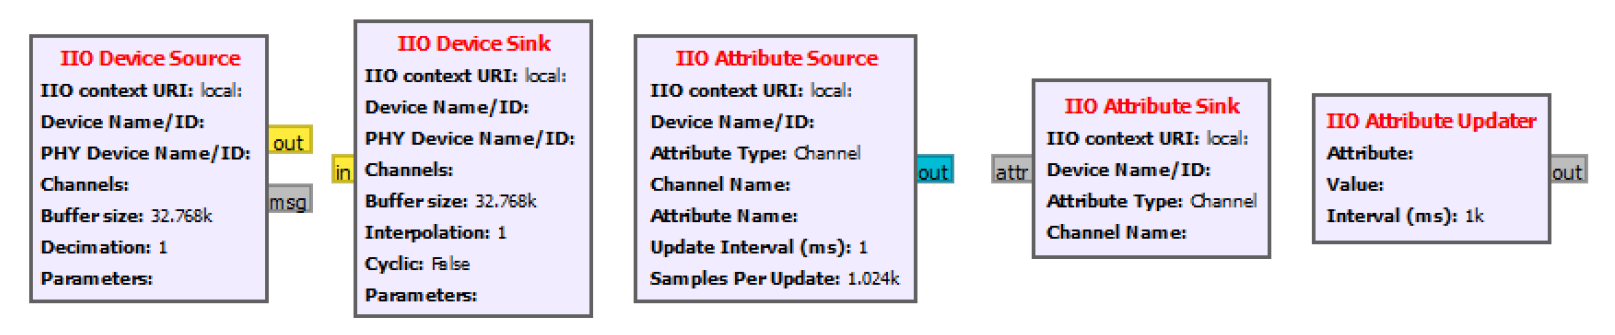
\includegraphics[width=0.8\textwidth]{generic_iio_blocks.png}}}
	\caption{Generic IIO Blocks with Default Values}
	\label{fig::generic_iio_blocks}
\end{figure}

After replacing the PlutoSDR source and sink blocks with the blocks shown in Figure \ref{fig::generic_iio_blocks}, we repeat the experiment from Section \ref{section::gnu_radio_loopback}. Then, we change the TX and RX frequencies from 2.4 GHz to 915 MHz and increase the sample rates from 2.084 MSPS to a higher arbitrarily-chosen sampling rate. Finally, we verify that each of these settings are correctly applied using IIO Scope plugins and the \texttt{iio\_attr} command. 
 
\section{Results}
\subsection{Industrial Input/Output (IIO)}

In this section, we display the results from the industrial input/output commands provided in Section \ref{section::industrial_input_output}. Figure \ref{fig::iio_info_putty} displays the results of the \texttt{iio\_info -s} command, when executed in Putty (an SSH terminal).  

\begin{figure}[H]
	\centerline{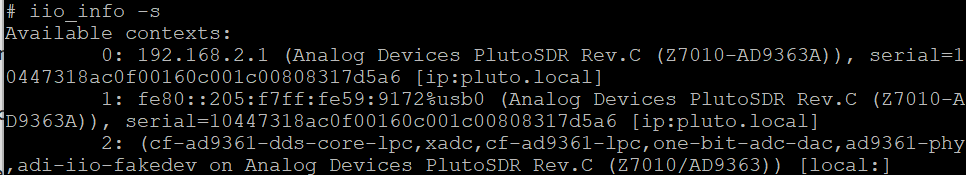
\includegraphics[width=0.9\textwidth]{iio_info_putty.png}}
	\caption{Result of \texttt{iio\_info -s} Command when Executed in Putty}
	\label{fig::iio_info_putty}
\end{figure}

Figure \ref{fig::iio_info_cmd} shows the outputs of the same command when executed in command prompt, a local PC terminal.

\begin{figure}[H]
	\centerline{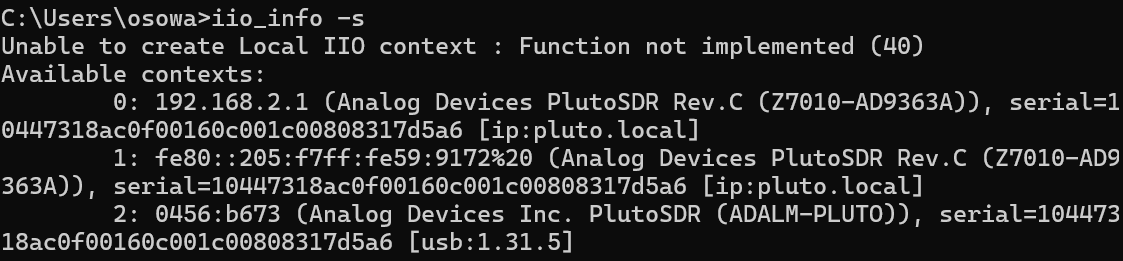
\includegraphics[width=0.9\textwidth]{iio_info_cmd.png}}
	\caption{Result of \texttt{iio\_info -s} Command when Executed in Command Prompt}
	\label{fig::iio_info_cmd}
\end{figure}

Compared to the outputs shown in Figure \ref{fig::iio_info_putty}, the command prompt output shows very similar URIs. Both contain an ip:pluto.local URI with an IP address of 192.168.2.1. They also both contain an additional ip:pluto.local URI, which is nearly the same. However, the biggest difference between the two outputs is in the final URI. The SSH output shows a local URI (local:), while the command prompt output shows a USB URI (usb:1.31.5). We note that command prompt also contains an additional warning message, which says "Unable to create Local IIO context: Function not implemented (40)." This warning message is described in more detail in \cite{analog_devices_libiio_error}. However, it is expected warning because \texttt{iio\_info} tries to open local contexts, which are not supported in Windows. For comparison, we run the same command on the Virtual Machine. The results of this command are display in Figure \ref{fig::iio_info_vm}.

\begin{figure}[H]
	\centerline{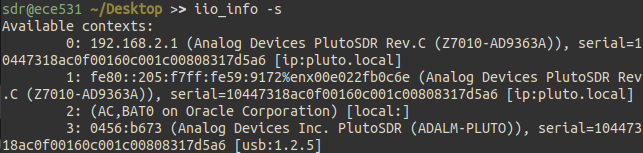
\includegraphics[width=0.9\textwidth]{iio_info_vm.png}}
	\caption{Result of \texttt{iio\_info -s} Command when Executed in Virtual Machine}
	\label{fig::iio_info_vm}
\end{figure}

Compared to the results of Figure \ref{fig::iio_info_cmd}, we see that the IIO context warning message is no longer present. Next, we use the \texttt{iio\_attr -d} command without a device to list all the devices. The output of this command is listed in Figure \ref{fig::iio_devices}.

\begin{figure}[H]
	\centerline{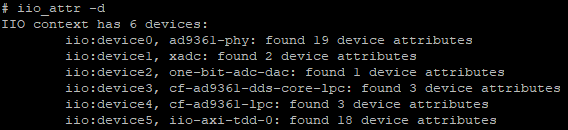
\includegraphics[width=0.75\textwidth]{iio_devices.png}}
	\caption{List of IIO Devices}
	\label{fig::iio_devices}
\end{figure}

Examining the command output, we find that \textit{ad9361-phy} corresponds to iio:device0. With the following command, we can get the name of iio:device0 and confirm our findings:

\begin{center}
\texttt{cat /sys/bus/iio/devices/iio:device0/name}
\end{center}

The outputs of this command are given in Figure \ref{fig::iio_device0_name}.

\begin{figure}[H]
	\centerline{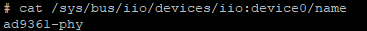
\includegraphics[width=0.5\textwidth]{iio_device0_name.png}}
	\caption{Confirming Name of ``iio:device0"}
	\label{fig::iio_device0_name}
\end{figure}

Examining the command outputs, we find that the name of iio:device0 is \textit{ad9361-phy} as expected. We can pass the name of the device as an argument to the \text{iio\_attr -d} command to list the attributes of the device. The results of this command are given in Figure \ref{fig::iio_raw_attributes}.

\begin{figure}[H]
	\centerline{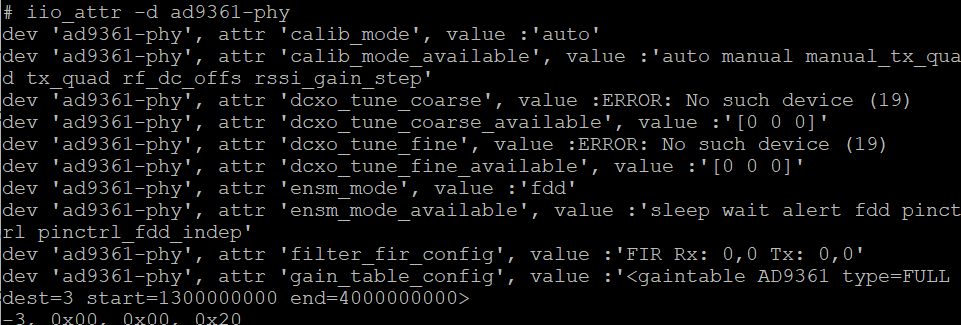
\includegraphics[width=0.9\textwidth]{iio_raw_attributes.png}}
	\caption{Attributes for the \textit{ad9361-phy} Device}
	\label{fig::iio_raw_attributes}
\end{figure}

This command gives the device attributes and their values. However, the command window is very cluttered. We can extract just the attribute names from the command output using a combination of \texttt{grep} and \texttt{sed} as illustrated in Figure \ref{fig::iio_filtered_attributes}.

\begin{figure}[H]
	\centerline{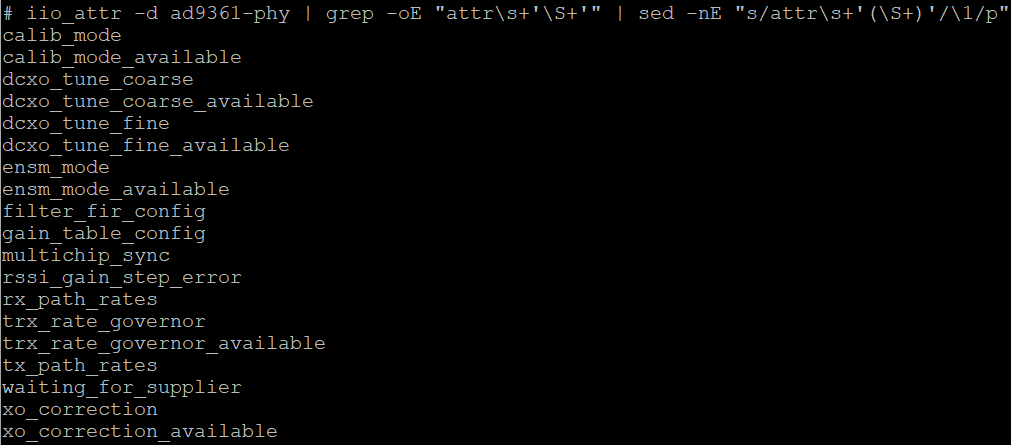
\includegraphics[width=0.9\textwidth]{iio_filtered_attributes.png}}
	\caption{Filtering Output of \texttt{iio\_attr} Command}
	\label{fig::iio_filtered_attributes}
\end{figure}

TODO: NEED TO ADD WHAT THE AD9361-PHY DOES!

% Results and discussion of the laboratory experiment, including captured outputs, observations, and responses to laboratory questions.

\subsection{GNU Radio Loopback}

We use the GNU Radio flowchart shown in Figure \ref{fig::gnu_radio_loopback_flowchart0} to perform a loopback test. We start the experiment by reviewing the properties of the PlutoSDR blocks (both transmit and receive). Relevant properties for each block are displayed in Figures \ref{fig::general_attributes_pluto_sdr_sink} - \ref{fig::filter_attributes_pluto_sdr_source}.

\begin{figure}[H]
	\centerline{\fbox{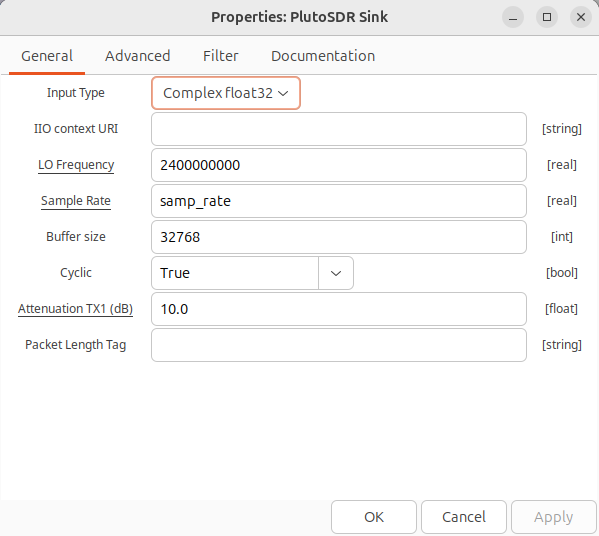
\includegraphics[width=0.5\textwidth]{general_attributes_pluto_sdr_sink.png}}}
	\caption{General Attributes of Pluto SDR Sink}
	\label{fig::general_attributes_pluto_sdr_sink}
\end{figure}

\begin{figure}[H]
	\centerline{\fbox{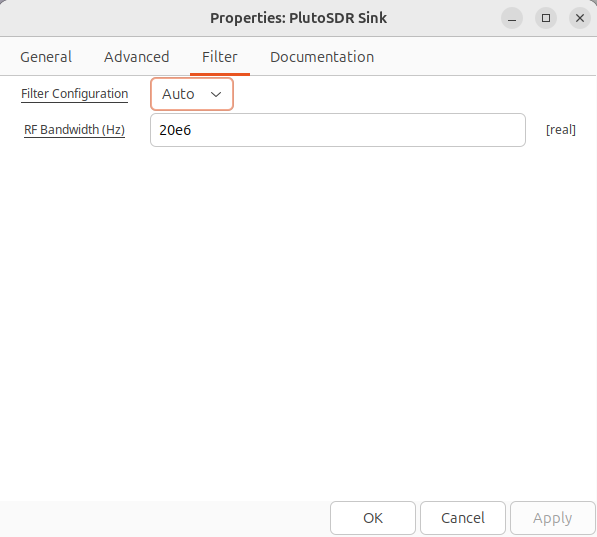
\includegraphics[width=0.5\textwidth]{filter_attributes_pluto_sdr_sink.png}}}
	\caption{Filter Attributes of Pluto SDR Sink}
	\label{fig::filter_attributes_pluto_sdr_sink}
\end{figure}

\begin{figure}[H]
	\centerline{\fbox{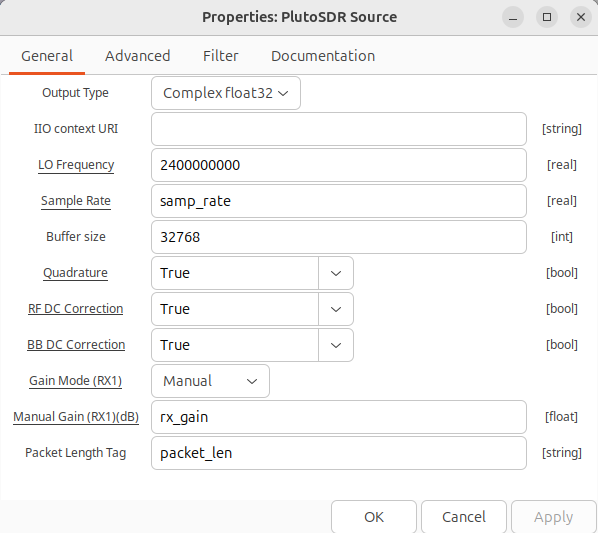
\includegraphics[width=0.5\textwidth]{general_attributes_pluto_sdr_source.png}}}
	\caption{General Attributes of Pluto SDR Source}
	\label{fig::general_attributes_pluto_sdr_source}
\end{figure}

\begin{figure}[H]
	\centerline{\fbox{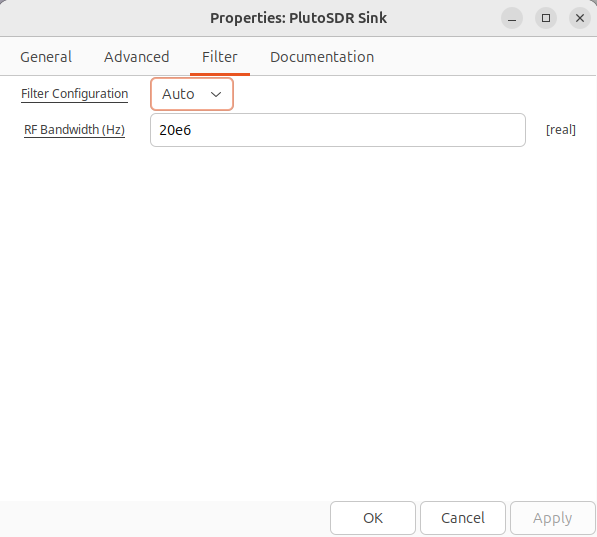
\includegraphics[width=0.5\textwidth]{filter_attributes_pluto_sdr_sink.png}}}
	\caption{Filter Attributes of Pluto SDR Source}
	\label{fig::filter_attributes_pluto_sdr_source}
\end{figure}

The RF bandwidth sets the bandwidth of the analog filters in the TX and RX paths. It is set at 20 MHz in Figure \ref{fig::filter_attributes_pluto_sdr_sink} and \ref{fig::filter_attributes_pluto_sdr_source}. The TX filter removes sampling artifacts and acts as a low-pass filter prior to upconversion. When we mix the signal, we are centering a copy of the spectrum at $+f_c$ and $-f_c$. If our signal is not properly bandlimited, the spectral copies may add together resulting in distortion. The RX filter is responsible for getting rid of the unwanted mixer products and removing out-of-band noise prior to sampling. If our filter bandwidth is too large, this unwanted noise will alias into our spectrum, degrading the SNR. 

Next, we review the cyclic option in the PlutoSDR sink. When the cyclic option is selected, as illustrated in Figure \ref{fig::general_attributes_pluto_sdr_sink}, the PlutoSDR will repeat the first buffer of samples it receives until the program is stopped. Conversely, when this option is not selected, the PlutoSDR will transmit buffers of samples as it receives them, creating a potentially discontinuous stream, which is more difficult to analyze. Additionally, not re-transmitting the same buffer of samples enables us to dedicate more of the USB bandwidth to the received data stream. As long as our buffer size is a multiple of the period, the cyclic option results in the same transmission as a signal source feeding a PlutoSDR Sink with infinite USB bandwidth.

The manual gain control in the PlutoSDR source block disables AGC and allows us to manually set the attenuation. Alternative gain control strategies include manual, slow attack, hybrid, and fast attack. The hybrid gain control is present in just the GNU Radio block and can be set view \texttt{iio\_attr}. However, it is not present in the MATLAB API. The hybrid mode is the same as the slow attack AGC mode with the exception of the gain update counter, which is not present in hybrid mode. This allows the hybrid algorithm to more frequently adjust the attenuation.

Using the default receive gain setting of 20 dB, we observe the time and frequency data shown in Figure \ref{fig::gnu_radio_loopback_baseline}.

\begin{figure}[H]
	\centerline{\fbox{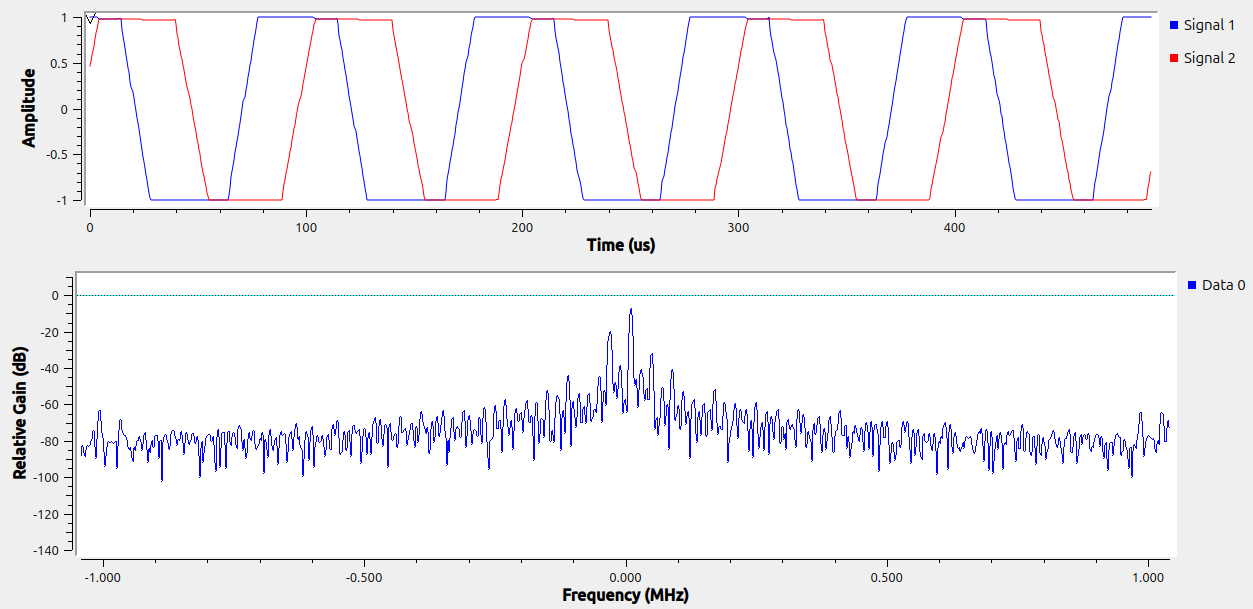
\includegraphics[width=0.8\textwidth]{gnu_radio_loopback_baseline.png}}}
	\caption{Baseline Loopback Test with GNU Radio}
	\label{fig::gnu_radio_loopback_baseline}
\end{figure}

With the default settings the signal has already clipped. We can reduce the receive signal gain until we no longer see distortion. Figure \ref{fig::gnu_radio_loopback_rx_gain_12dB} shows the collect with 12 dB of receive signal gain.

\begin{figure}[H]
	\centerline{\fbox{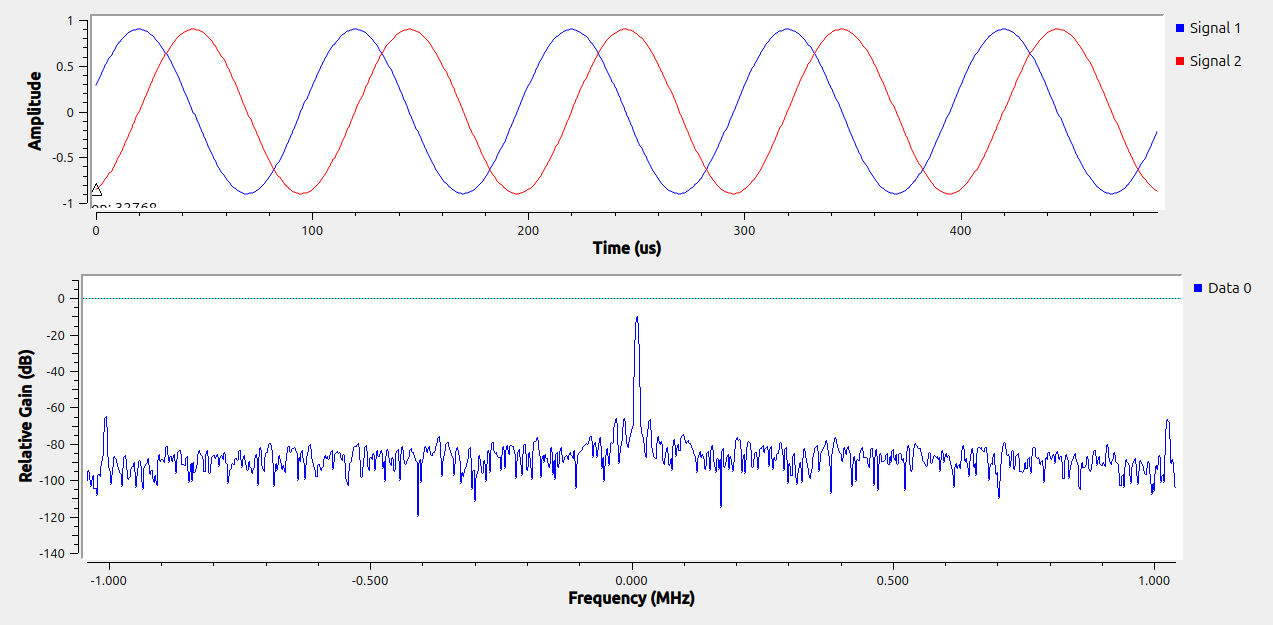
\includegraphics[width=0.8\textwidth]{gnu_radio_loopback_rx_gain_12dB.png}}}
	\caption{GNU Radio Loopback Collect with 12 dB of RX Gain}
	\label{fig::gnu_radio_loopback_rx_gain_12dB}
\end{figure}

We note that the signal is no longer distorted but is very close to full scale ($\pm 1$). If we increase the receive signal gain back up to 13 dB, we start to see clipping again as illustrated in Figure \ref{fig::gnu_radio_loopback_rx_gain_13dB}.

\begin{figure}[H]
	\centerline{\fbox{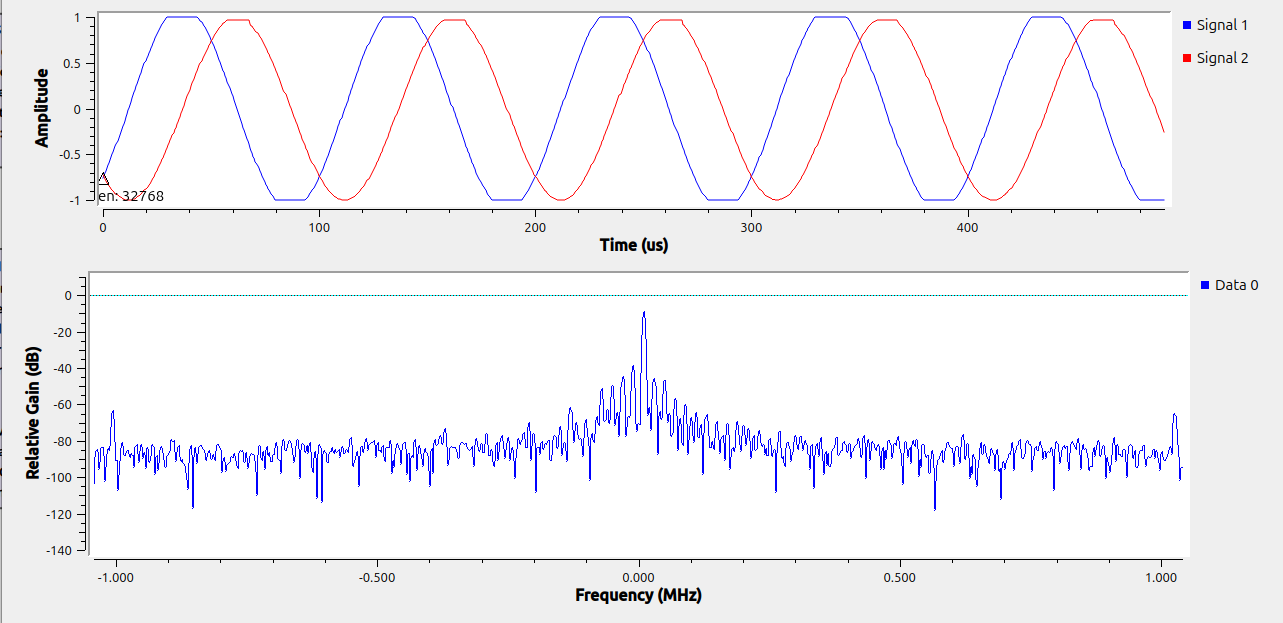
\includegraphics[width=0.8\textwidth]{gnu_radio_loopback_rx_gain_13dB.png}}}
	\caption{GNU Radio Loopback Collect with 13 dB of RX Gain}
	\label{fig::gnu_radio_loopback_rx_gain_13dB}
\end{figure}

Next, we replace the "QT Time Sink" and "QT Frequency Sink" sink and observe the output. Figure \ref{fig::gnu_radio_loopback_qt_gui_sink} shows the frequency response with the RX Gain set to 0 dB.

\begin{figure}[H]
	\centerline{\fbox{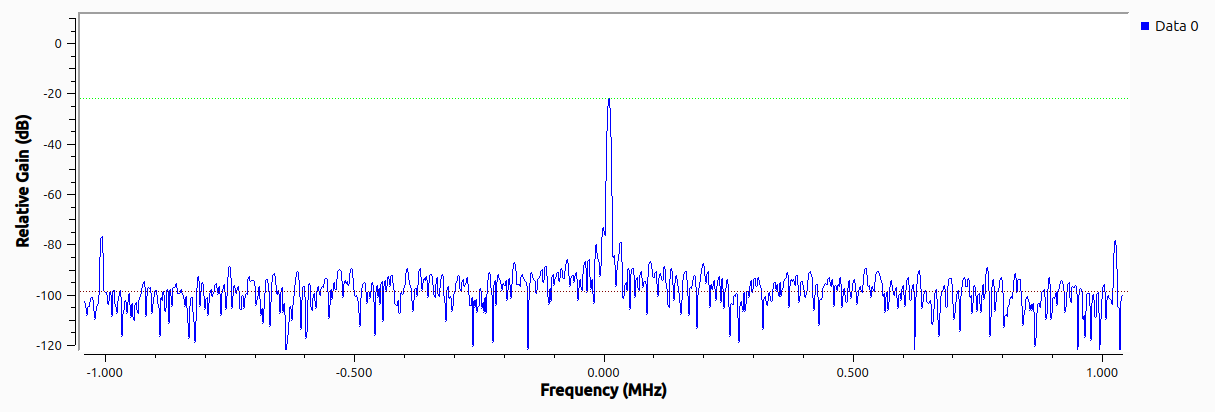
\includegraphics[width=0.8\textwidth]{gnu_radio_loopback_qt_gui_sink.png}}}
	\caption{Frequency Response with QT GUI Sink and 0 dB of RX Gain}
	\label{fig::gnu_radio_loopback_qt_gui_sink}
\end{figure}

Looking at the frequency response, we see roughly 75 dB of SNR (peak to noise floor). Figure \ref{fig::gnu_radio_loopback_qt_gui_sink} shows the frequency response for the same configuration, average in amplitude over 256 frames.

\begin{figure}[H]
	\centerline{\fbox{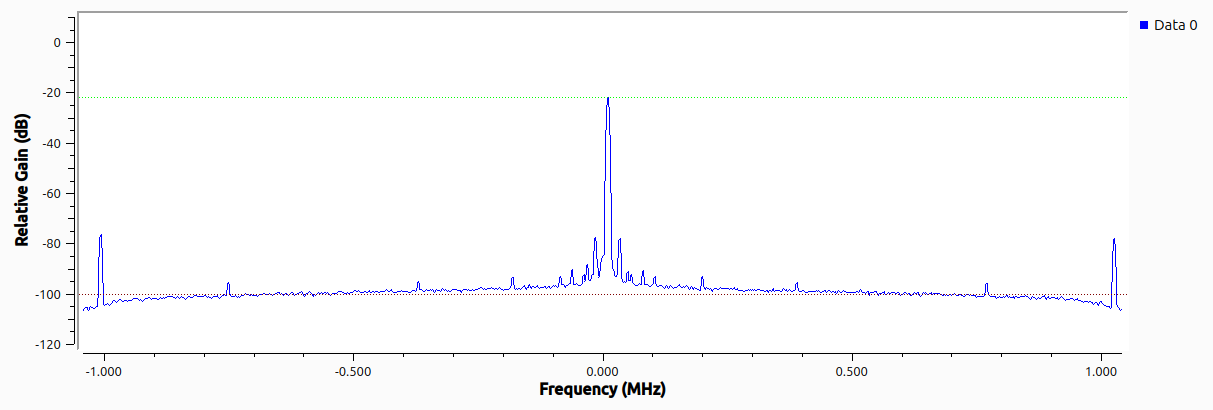
\includegraphics[width=0.8\textwidth]{gnu_radio_loopback_qt_gui_sink_avg_256.png}}}
	\caption{Frequency Response Averaged Over 256 Frames}
	\label{fig::gnu_radio_loopback_qt_gui_sink_avg_256}
\end{figure}

Comparing Figures \ref{fig::gnu_radio_loopback_qt_gui_sink} and \ref{fig::gnu_radio_loopback_qt_gui_sink_avg_256}, we see that integrating multiple frames of the FFT output reduces the variance of the noise, allowing us to better visualize sidelobes in the frequency response. 

Using a different window will change the sidelobe levels and sidelobe rolloff in the frequency response. However, when we reduce sidelobe levels we also increase the mainlobe width. Compare Figure \ref{fig::gnu_radio_loopback_qt_gui_sink_avg_256} which uses a Blackman-harris window to Figure \ref{fig::gnu_radio_loopback_qt_gui_sink_rect_win} which uses a rectangular window. The sidelobes of the Blackman-harris are substantially lower. However, the mainlobe of the frequency response is much larger.

\begin{figure}[H]
	\centerline{\fbox{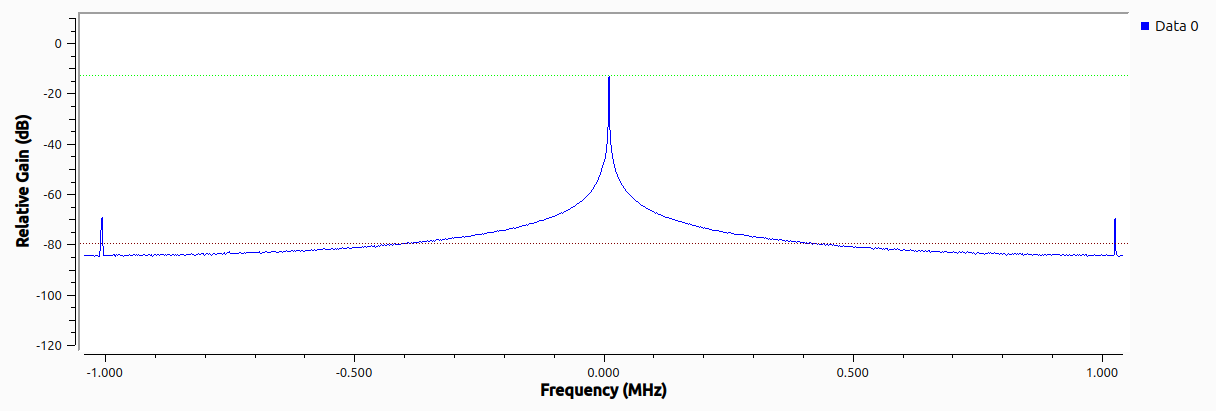
\includegraphics[width=0.8\textwidth]{gnu_radio_loopback_qt_gui_sink_rect_win.png}}}
	\caption{Frequency Response Using Rectangular Window Instead of Blackman-Harris Window}
	\label{fig::gnu_radio_loopback_qt_gui_sink_rect_win}
\end{figure}

The PlutoSDR uses a quadrature mixer to mix the DAC output to the correct frequency. The output of a quadrature mixer is given as follows:

\begin{align}
	y(t) &= \cos(2{\pi}f_ct)\text{Re}\{x(t)\} - \sin(2{\pi}f_ct)\text{Im}\{x(t)\} \\ [3pt]
	&= \text{Re}\{(\text{Re}\{x(t)\} + j\text{Im}\{x(t)\})(\cos(2{\pi}f_ct) + j\sin(2{\pi}f_ct))\} \\ [3pt]
	&= \text{Re}\{X(t)e^{j2{\pi}f_ct}\}
\end{align}

In other words, the transmitted spectrum should be centered about $f_c$, and the frequency image should be centered about $-f_c$. For our experiment, we output a 10 kHZ sinusoid and mixed it with a 2.4 GHz LO. Thus, our transmitted frequency was 2.40001 GHz.

\section{Conclusion}
% Conclusions to the overall lab that discuss meaningful lessons learned and other takeaways from the assignment. (Important)

\nocite{analog_devices_libiio_error}
\bibliographystyle{IEEEtran}
\bibliography{sources}{}
%\bibliographystyle{ieeetr}
	
\end{document}